\documentclass[border=15pt]{standalone}
\usepackage{amsmath, amssymb}
\usepackage{tikz}
\usetikzlibrary{arrows.meta}

\definecolor{block0}{HTML}{E53935}
\definecolor{block1}{HTML}{1E88E5}
\definecolor{block2}{HTML}{43A047}
\definecolor{block3}{HTML}{FB8C00}

\begin{document}
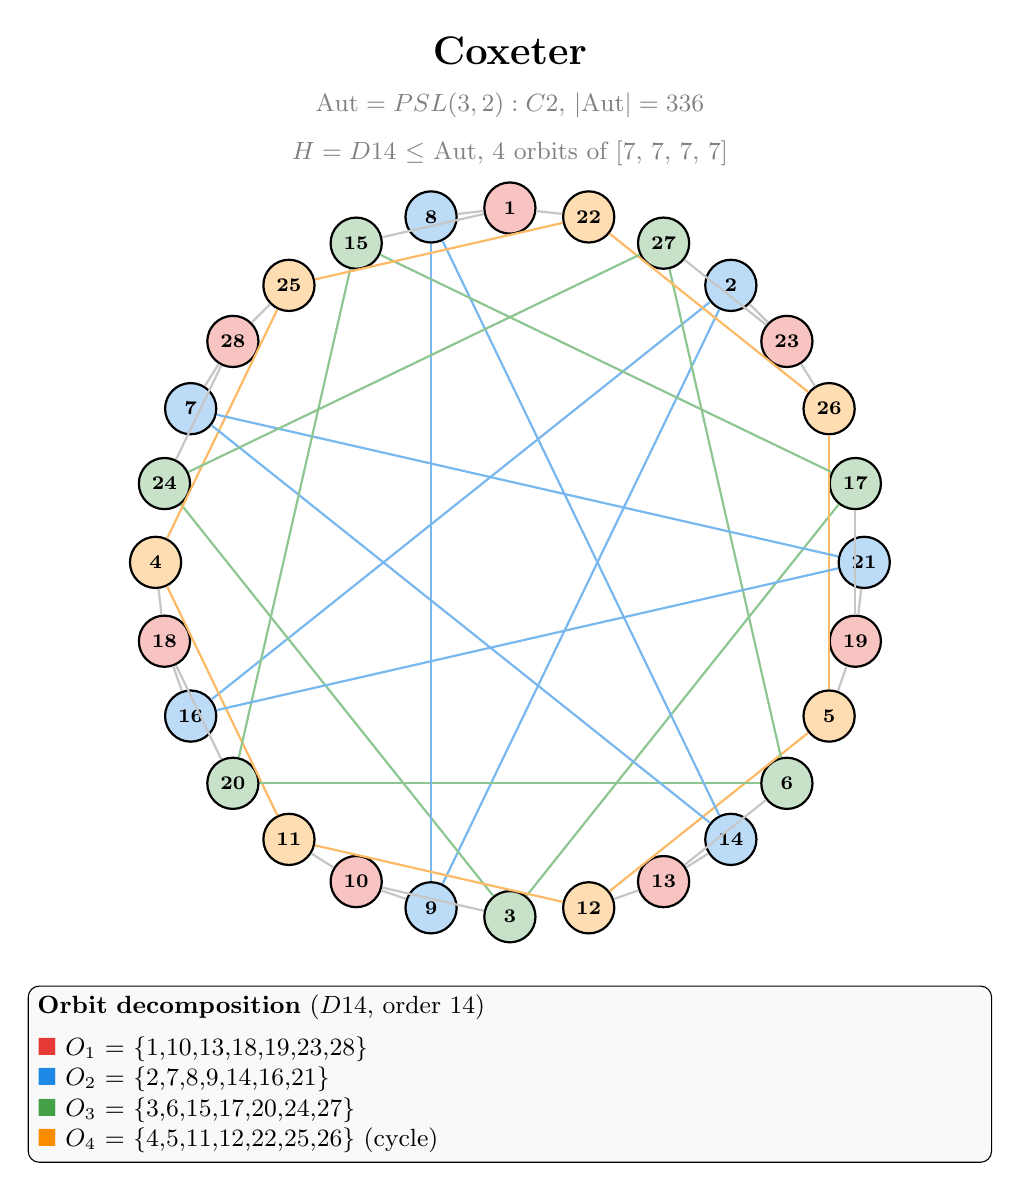
\begin{tikzpicture}[
  vertex/.style={circle, draw, thick, minimum size=6.5mm, inner sep=0pt,
                 font=\scriptsize\bfseries},
  edge/.style={thick, gray!45},
  title/.style={font=\Large\bfseries},
  subtitle/.style={font=\small, text=gray},
]

\node[title] at (0, 6.5) {Coxeter};
\node[subtitle] at (0, 5.8) {$\mathrm{Aut} = PSL(3,2) : C2$, $|\mathrm{Aut}| = 336$};
\node[subtitle] at (0, 5.2) {$H = D14$ $\leq$ $\mathrm{Aut}$, 4 orbits of [7, 7, 7, 7]};

\node[vertex, fill=block0!30] (v1) at (0.000, 4.500) {1};
\node[vertex, fill=block1!30] (v2) at (2.806, 3.518) {2};
\node[vertex, fill=block2!30] (v3) at (-0.000, -4.500) {3};
\node[vertex, fill=block3!30] (v4) at (-4.500, 0.000) {4};
\node[vertex, fill=block3!30] (v5) at (4.054, -1.952) {5};
\node[vertex, fill=block2!30] (v6) at (3.518, -2.806) {6};
\node[vertex, fill=block1!30] (v7) at (-4.054, 1.952) {7};
\node[vertex, fill=block1!30] (v8) at (-1.001, 4.387) {8};
\node[vertex, fill=block1!30] (v9) at (-1.001, -4.387) {9};
\node[vertex, fill=block0!30] (v10) at (-1.952, -4.054) {10};
\node[vertex, fill=block3!30] (v11) at (-2.806, -3.518) {11};
\node[vertex, fill=block3!30] (v12) at (1.001, -4.387) {12};
\node[vertex, fill=block0!30] (v13) at (1.952, -4.054) {13};
\node[vertex, fill=block1!30] (v14) at (2.806, -3.518) {14};
\node[vertex, fill=block2!30] (v15) at (-1.952, 4.054) {15};
\node[vertex, fill=block1!30] (v16) at (-4.054, -1.952) {16};
\node[vertex, fill=block2!30] (v17) at (4.387, 1.001) {17};
\node[vertex, fill=block0!30] (v18) at (-4.387, -1.001) {18};
\node[vertex, fill=block0!30] (v19) at (4.387, -1.001) {19};
\node[vertex, fill=block2!30] (v20) at (-3.518, -2.806) {20};
\node[vertex, fill=block1!30] (v21) at (4.500, -0.000) {21};
\node[vertex, fill=block3!30] (v22) at (1.001, 4.387) {22};
\node[vertex, fill=block0!30] (v23) at (3.518, 2.806) {23};
\node[vertex, fill=block2!30] (v24) at (-4.387, 1.001) {24};
\node[vertex, fill=block3!30] (v25) at (-2.806, 3.518) {25};
\node[vertex, fill=block3!30] (v26) at (4.054, 1.952) {26};
\node[vertex, fill=block2!30] (v27) at (1.952, 4.054) {27};
\node[vertex, fill=block0!30] (v28) at (-3.518, 2.806) {28};

\draw[edge] (v1) -- (v8);
\draw[edge] (v1) -- (v15);
\draw[edge] (v1) -- (v22);
\draw[thick, block1!60] (v2) -- (v9);
\draw[thick, block1!60] (v2) -- (v16);
\draw[edge] (v2) -- (v23);
\draw[edge] (v3) -- (v10);
\draw[thick, block2!60] (v3) -- (v17);
\draw[thick, block2!60] (v3) -- (v24);
\draw[thick, block3!60] (v4) -- (v11);
\draw[edge] (v4) -- (v18);
\draw[thick, block3!60] (v4) -- (v25);
\draw[thick, block3!60] (v5) -- (v12);
\draw[edge] (v5) -- (v19);
\draw[thick, block3!60] (v5) -- (v26);
\draw[edge] (v6) -- (v13);
\draw[thick, block2!60] (v6) -- (v20);
\draw[thick, block2!60] (v6) -- (v27);
\draw[thick, block1!60] (v7) -- (v14);
\draw[thick, block1!60] (v7) -- (v21);
\draw[edge] (v7) -- (v28);
\draw[thick, block1!60] (v8) -- (v9);
\draw[thick, block1!60] (v8) -- (v14);
\draw[edge] (v9) -- (v10);
\draw[edge] (v10) -- (v11);
\draw[thick, block3!60] (v11) -- (v12);
\draw[edge] (v12) -- (v13);
\draw[edge] (v13) -- (v14);
\draw[thick, block2!60] (v15) -- (v17);
\draw[thick, block2!60] (v15) -- (v20);
\draw[edge] (v16) -- (v18);
\draw[thick, block1!60] (v16) -- (v21);
\draw[edge] (v17) -- (v19);
\draw[edge] (v18) -- (v20);
\draw[edge] (v19) -- (v21);
\draw[thick, block3!60] (v22) -- (v25);
\draw[thick, block3!60] (v22) -- (v26);
\draw[edge] (v23) -- (v26);
\draw[edge] (v23) -- (v27);
\draw[thick, block2!60] (v24) -- (v27);
\draw[edge] (v24) -- (v28);
\draw[edge] (v25) -- (v28);

\node[draw, rounded corners, fill=gray!5, text width=12cm, align=left, font=\small]
  at (0, -6.5) {
  \textbf{Orbit decomposition} ($D14$, order 14) \\[4pt]
  \textcolor{block0}{$\blacksquare$} $O_{1}$ = \{1,10,13,18,19,23,28\} \\
  \textcolor{block1}{$\blacksquare$} $O_{2}$ = \{2,7,8,9,14,16,21\} \\
  \textcolor{block2}{$\blacksquare$} $O_{3}$ = \{3,6,15,17,20,24,27\} \\
  \textcolor{block3}{$\blacksquare$} $O_{4}$ = \{4,5,11,12,22,25,26\} (cycle)
};

\end{tikzpicture}
\end{document}